\documentclass{article}
\usepackage[utf8]{inputenc}
\usepackage{graphicx}
\usepackage{sectsty}


\title{Game Design Document}
\author{Group 4: Pico Bello B.V.}
\date{27-11-2014}


\begin{document}
	\fontencoding{T1}\fontfamily{lmss}\fontseries{m}\selectfont

	\allsectionsfont{\fontfamily{lmss}\selectfont}


	\maketitle
	\begin{figure}[ht!]
		\centering
		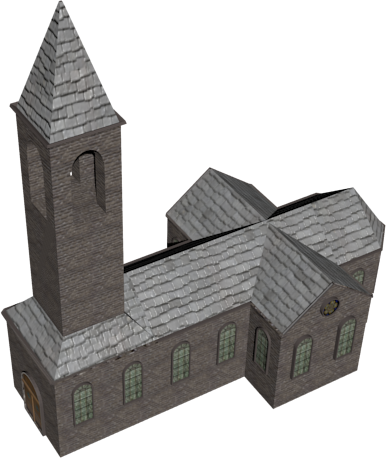
\includegraphics[width=100mm]{images/Front.png}
	\end{figure}
	\newpage
\subsection*{Project Name}
	\qquad Awesome Spel
\subsection*{Team Name}
	\qquad Group 4: Pico Bello B.V.
\subsection*{Team Members}
	\begin{itemize}
		\item \textbf{Thomas de Boer}, Game Designer
		\item \textbf{Luuk de Niet}, Lead Artist
		\item \textbf{Boyd Verdoorn}, Lead Programmer
		\item \textbf{Rense Wisse}, World Builder
		\item \textbf{Jesper Spillenaar Bilgen}, Producer
	\end{itemize}

	\newpage

\section{Introduction}
	Awesome Spel is a game that is based around the old Film Noir movie genre, but with a modern twist. The game will be in color, albeit a bit grimey. The player should solve a hideous murder, while playing as a detective, George Carter. There are several ways to collect evidence, by searching for clues, interrogation and exploration.

	\subsection{How and Why?}
		This game is being developed as part of an assignment for the TU Delft in the Netherlands. We are required to use Unity 4.6 and Blender as development tools. Other tools we use are Crazybump, for creating bump maps, audacity as a audio suite and LaTeX for Deliverables. The teams for the assignment were put together based on experience in different fields. We don't have any team members with a design background, so this is a small hurdle. We try to overcome this by working on the models with a large part of the team.

	\subsection{Inspiration}
		Our Inspiration was games such as LA noire, Ace Attorney and The Walking Dead, story based exploration games, where the outcome changes depending on the choices made by the player.\\
		The orthographic platform styled level design was inspired by bastion and similar games.\\
		The art style and setting are mostly inspired by Bioshock Infinite and the movie Blade Runner.
\section{Target Audience}
	\begin{itemize}
		\item Male
		\item 16 to 25 years old
		\item Likes Games
		\item Likes TV Series
		\item Uses the Steam Platform
		\item Casual Gamer
	\end{itemize}
	We are targeting casual to midrange gamers, who are interested in an story based interactive experience. Because our game relies quite a bit on story, it can pique the interest of people who watch a lot of series. The age group is Teen to Young Adult, because some of the themes may not be suitable for younger children. Although we target young males, we think our game has aspects that will appeal to a larger audience.


\section{Platform \& Controls}
	The game is developed for PC, with mac as a possible addition. We use the mouse and keyboard as control devices, because the mouse has the ability to precisely point at objects. This gives the player more control over the game. If there were more time, we believe creating the game for mobile platforms, such as Android, iOS and Windows Phone, would appeal to a large crowd of casual mobile players, who are willing to buy this type of games. This is however not something that is within the scope of our project at the moment.

\section{Story, Characters and setting of the game}
	\subsection{Setting}
		The story is set in a american metropolis in the early 50's. We want to emphasize brown brick houses, the darkness of the bad neighbourhoods in the city and the large amount of crime. 
	\subsection{Story and Main Characters}
		The game is based around a single story of a murder case. 
		\begin{quote}
			You are a businessman with a workaholic attitude, but a dark past. This is the day your past catches up to you. There is someone in your apartment. You try to run and escape from the madness that is now your reality. But it is to no avail.
		\end{quote}
		The story is told through different perpectives, each with their own destinctive gameplay and design. 
		\begin{quote}
			You are George Carter. A policeman, as clean as they come these days. There’s been a suicide, probably another overworked and coked up businessman again. It’s happening more often these days, since the economy went mad. It’s not been a happy couple of years, with your wife leaving and these suicides taking away all the joy. You go to the apartment. It’s a shabby old place, but nothing too bad. You’ve seen worse, much worse. The moment you get in something seems off. There is something that’s not as it seems.
		\end{quote}
		It's told three times in total, each time giving more information about the murder. 
		\begin{quote}
			You are a young, upcoming journalist for a tabloid newspaper. You’ve been trying to get the good stuff. Corruption in Politics, Hardship on the streets and Murder in the Underworld, . All they’ve given you so far is the record for biggest pizza and a dog beauty pageant. It’s not always easy to start at the bottom. Your boss comes to your desk. He looks glum. “I’ve got a real assignment for you.” It’s a look like suicide, but the police say otherwise. It’s supposed to be a big piece in tomorrow’s newspaper. You go investigate.
		\end{quote}
		There are three roles: Detective, Journalist, and an undetermined family member.\\ \\
		\noindent
		The game concludes in a finale, where, depending on the choices of the player, the killer is apprehended. The game is a sort of 'third person investigation' and is played by walking around in the scene with the arrow keys and collecting evidence by clicking on different objects to investigate them. In the end it will become clear who the killer is, if the player has gathered enough evidence. Who the killer is will remain a secret, even for our supervisors ;). The characters will converge, but too little evidence may leave a character behind. We let the player play a short while with each character to make sure he knows everyone again. One central location, where everything is revealed and a final twist is given. \\ \\
		\noindent
		The Story is a pretty large part of our game, however we have given it a \textbf{low priority}, because it is not one of the programming components that will influence the technical difficulty, and therefor the grade. We are currently working with an 'smaller' version of the initial story, where only the detective is playable. We have eliminated some of our original side characters and put less time into elaborating the original story. If we have time left, we could make the decision to elaborate a bit more, but programming has a higher priority.
	\subsection*{Non Player Characters}
		We will use a number of anonymous NPCs, such as police men, hotel personnel and pedestrians, these are mainly for atmosphere. Besides these characters, we have a small number of unique NPCs, such as the Police Chief, a Priest and relatives of the victim, that can be interrogated. This could give the player more information about the story.
\section{Artificial Intelligence}
	We use A* to enable our Non Player Characters to wander around the city. These include Pedestrians and we could add cars, given enough time is at hand. A* will enable our pedestrians to follow a path and is ideal for use in 2D street maps, without tunnels or bridges.\\
	We will use a Neural Network to determine the outcome of the game, with the evidence collected as an input and one of several diffent endings as the ouput. If this does not work as expected, we will explore the possibilities of a different AI technique or just revert to a score based system.

\section{Level \& Environment Design}
	There are two basic level types in this game. The city and individual rooms.
	\subsection{City}
		We have a single city we can walk through and find hidden clues. The city is basically one large map with roads and buildings. On this map there are several landmarks, a church in a small park, the police station, a hotel and a hospital. These landmarks are always in the same location. The street plan is also premade. The buildings are procedurally generated on the startup of the game. The houses will be around 3 to 7 stories. There are street lights that will be placed automatically. We could also add procedurally placed clutter models, such as trash bags/cans and other junk. This will result in a better atmosphere.\\
		The player is free to roam this city. The city should feel big, but not so big that it becomes a chore to walk from A to B. If there is time we can allow the player to use automobiles to get around to circumvent this problem. We want Pedestrians to walk and Cars to drive around, so it gives the impression of a busy city.\\
		The camera is fixed to the player in a classic orthographic configuration, buildings become transparent if they are between the player and the camera, to allow the player better vision.
	\subsection{Indoors}
		These are individual rooms where the player can go to via the landmarks or events. These represent the indoor area of certain buildings. We will create several rooms, such as: The murder scene, a hotel room, the police chiefs office, the inside of the church etc. In these rooms there are clues to be found. The player can walk and click objects that may be clues. The atmosphere will rely heavily on the type of room. The police office will be clean and have the characteristic window blinds and a wooden desk. The crime scene will be darker, a bedroom, with a bed and more clutter. Stuff on the ground etc.

\section{Gameplay \& Mechanics}
		There are several ways to gain evidence. These can be seen as minigames.
		\begin{itemize}
			\item Interrogation. 
			This Minigame allows the player to interrogate suspects and witnesses. When the player asks more direct questions, the suspect will get more and more wary, to the point that the interrogation is over. This will force players to choose whether they want a few large pieces of info, rather than tiny chunks of info.
			\item Scanning for evidence.
			While indoors, the player can click on objects in a room to find out more about what happened. This is timed, so you have to think quickly.
			\item Investigation. By following leads, the player is lead to certain places on the world map where valuable information or clues are located. These leads come from clues and evidence and could be quite cryptic.
		\end{itemize}
\newpage
\section{Art}
	
	\subsection{Models}
		We use the MoSCow system for prioritizing the models.
	\begin{itemize}
		\item Humanoid models (M) - These are very important for the player and npc models. At least one male and one female model should be made, we can always scale these.
		\item Evidence models (M) - We need enough evidence to keep the player busy. Sigarette buds, weapons and the occasional red herring.
		\item Landmark models (M) - The church etc. These landmarks play a large part in the game.
		\item Building parts (M) - Windows, doors, fire escapes etc. for building generation.
		\item Furniture (M) - Beds, chairs, cupboards, tables etc. These will be used indoors to provide a proper setting for putting evidence in place.
		\item Park models (S) - We want to give the park a proper park feeling, with a couple of trees and bushes, but a green plain as underground could also work.
		\item Street Lights (S) - We will use these to give more atmosphere at night.
		\item Character Clothing items (S) -  - It is important to be able to discern the player from other characters, and the other characters from each other. These help and give a proper feeling for the time period at the same time.
		\item Clutter models (C) - Tin cans, trash, cars, all non essential models on the street. These will give much more life to the city.

	\end{itemize}

	\subsection{Textures}
		\begin{itemize}
			\item Several different humanoid textures (M) - To be able to discern between characters.
			\item Textures for models we made (M) - Most models need a texture to be recognizable.
			\item Roads (M) - The roads need textures to be recognizable.
			\item Road specular and bump maps (C) - These give much more depth and feeling to the streets.
			\item Dirt texture overlays (C) - Overlaying dirt over the buildings and roads makes them less repetitive.
		\end{itemize}


	\newpage
	We are aiming for a dark gritty retro city. Late 40's, early 50's style. Film Noire style. This includes a film grain and a lot of brown and greyscale textures. And of course hats.
	\begin{figure}[ht!]
		\centering
		\centerline{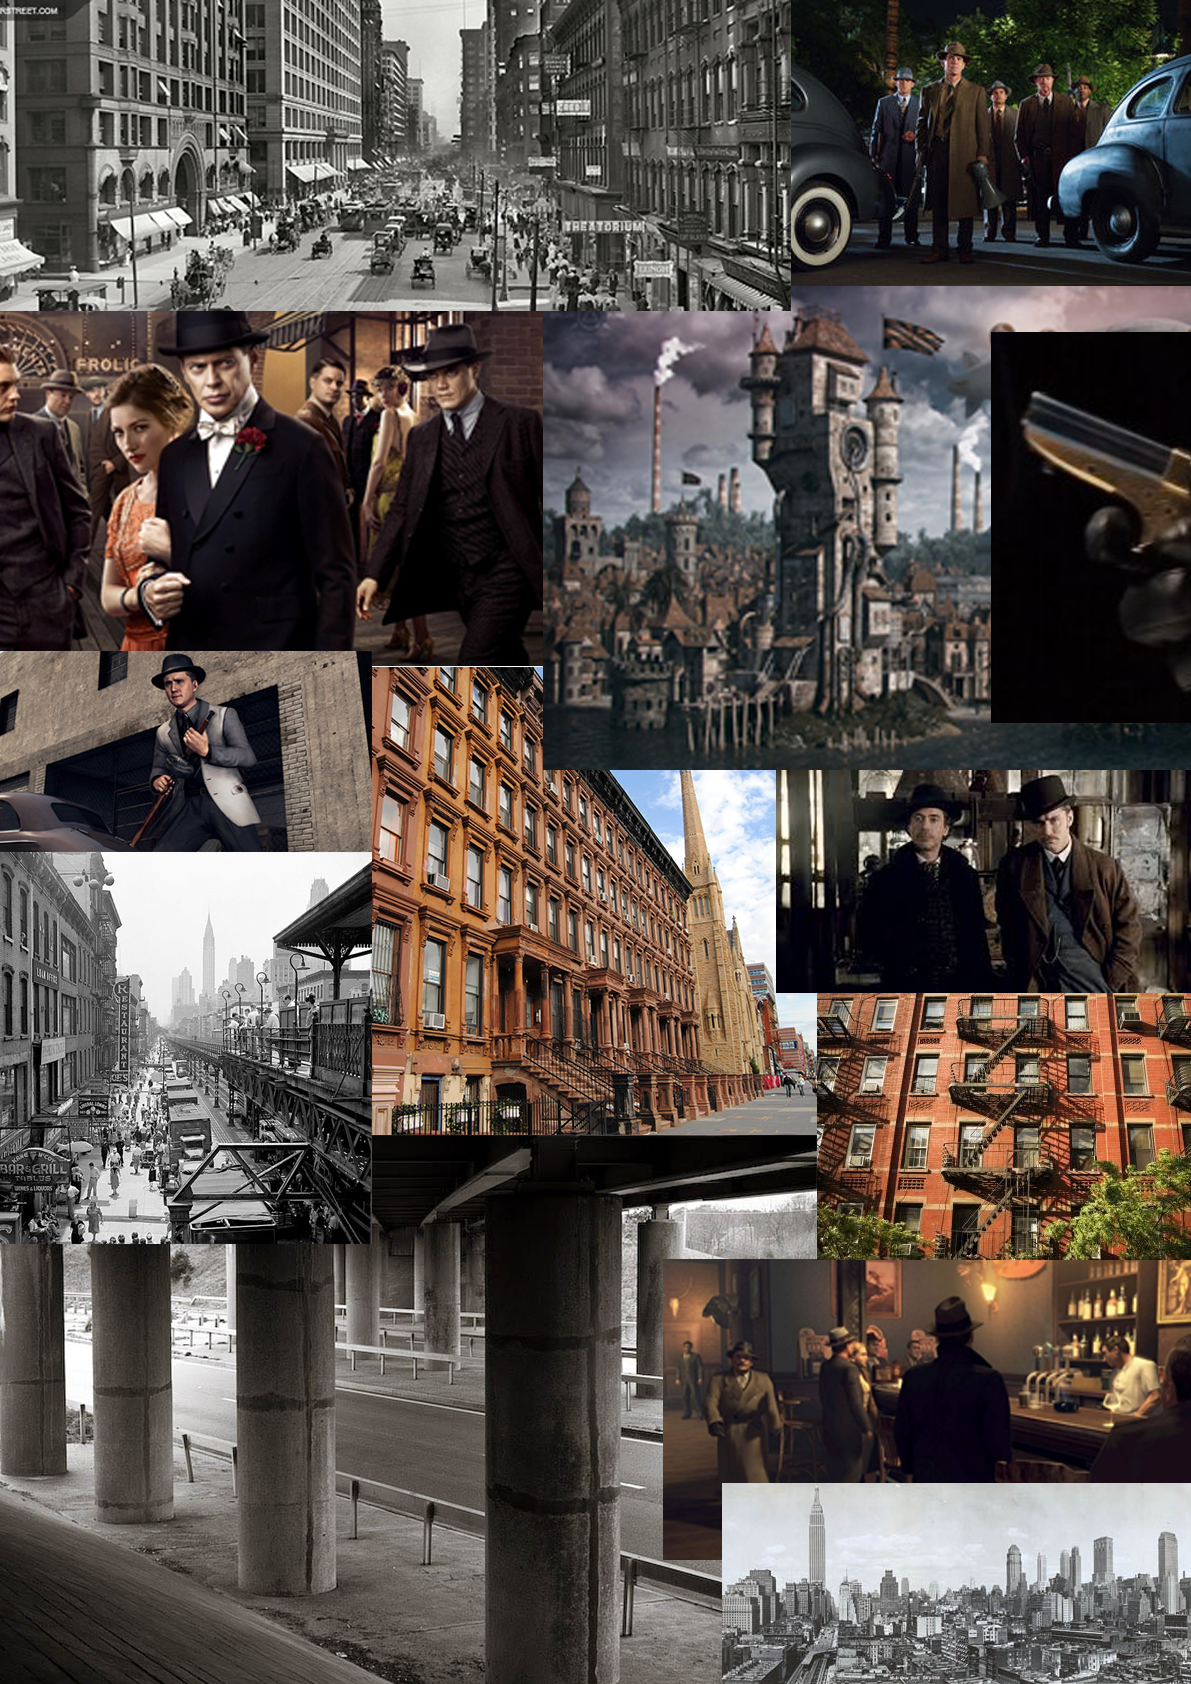
\includegraphics[width=120mm]{images/collage.png}}
	\end{figure}
	\newpage


\section{Sound of Music}
	Music will be sourced from websites that share music under a Creative Commons licence. The authors will be credited in the game. We are looking for music that is not too happy or glum, to convey the atmosphere better. We want to use 2 to 3 songs in the main game to make sure it doesn't get too repetitive. The songs should match as good as possible.\\
	SoundFX could be recorded by us as a strech goal. Otherwise we will use effects under CC licence as well. We need sounds for footsteps over different types of terrain. Picking up objects of different materials. etc.

\section{User interface \& Game controls}
	The player uses mouse and keyboard to operate the game. The WASD or arrow keys can be used to walk around. The mouse cursor is used to point at items or characters and we can left click for interaction with these objects.\\
	The game has the usual interface options, pauze/play menu, start menu. We want to have as few UI overlays in game as possible, to prevent breaking the immersion. The game is controlled with the mouse, so the cursor needs to be visible. We could create a custom mouse pointer. Inside the minigames we will use UI options to show time, character patience or other relevant information. When an item is found we will give a small popup box. The item is then placed in the inventory, where we can get an overview of all acquired items and the information associated with them.

\end{document}